\section{手首の3次元的な動きの推定に基づく刺身を切る動作の特徴量抽出}
本研究による提案手法は図\ref{fig:1}に示すとおり,スマートウォッチでセンシングを行なったデータから算出した3次元的な動きをもとに特徴量の抽出を行う.
先行研究\cite{kumazawaanalysis}では加速度のみを用いて推定するものもあるが,まな板との衝突時の加速度をもとに特徴量を抽出するため加速度変化の少ない静かな動作に弱い.
静かな動作のためにうまく取得できない例として刺身を切る動作があげられる.
そこで本研究では加速度・角速度センサから取得したデータをそのまま使用せず3次元的な動きを推定する.
3次元的な動きを使用すると奥から手前に腕を動かす動作をもとに特徴量を抽出できるようになる.

本研究では先ほど例にあげた刺身を切る動作の評価を対象とする.
切る動作から抽出をする特徴量は切った回数・切るペース・刃の角度である.
切った回数が身の分厚さ,切るペースが手際の良さ,刃の角度が切り方の評価基準となる.
他にも特徴量として扱えるデータは存在するが,検証のためこの3項目について検討を行う.


\figimage{images/fig1.pdf}{80}{本研究の概要図}{fig:1}

\subsection{データの収集}
本研究ではウェアラブルデバイスとしてスマートウォッチを使用した.
ウェアラブルデバイスの中にはセンサグローブやスマートリングなども存在している.
調理を対象とした動作の取得には指先の動作まで取得可能なセンサグローブが理想である.
しかし一般的に普及しておらず,専門家ではない一般の人を対象とする本研究には向かない.
一般に普及し,また料理という環境から防水性に優れたスマートウォッチを採用した.
センシングにはカメラを用いる手法も存在するが,本研究では使用しない.
理由として,調理動作中の手の動きは立体的な動きであるため,複数視点から撮影を行う必要がある.
そのためカメラを複数用意したり,位置を固定が必要になったりでデータ収集が複雑になり一般人に使わせるには難しいからである.

基本的な包丁の握り方では図\ref{fig:2}のようにウォッチの向きと包丁の刃の向きが連動する.
\figimage{images/fig2.pdf}{80}{スマートウォッチと刃の向きの連動}{fig:2}
スマートウォッチと包丁の動きは連動しているため,包丁を持つ側の手首の動きをセンシングしデータを収集する.
収集したデータは今後使用しやすいようにネットワークを介してオブジェクトストレージサーバへ蓄積する.
\subsection{3次元の動きの推定}
本研究では取得した角速度と加速度にMadgwickフィルタを用いてセンサフュージョンを行い,回転量をクォータニオンとして導出している.
他の候補としてカルマンフィルタがあるがモデルの構造が不明な場合に高精度を実現するのが難しい.
Madgwickフィルタは事前に求めておくべきパラメータが少なく処理が高速な特徴がある.
将来的にリアルタイムでの推定を見据え高精度なフィルタ処理と計算速度の観点からMadgwickフィルタを採用した.



クォータニオンとは回転の量を表すものである.
クォータニオンはオイラー角や回転行列と相互に変換可能であり,上下がわからなくなるジンバルロックという現象が発生しない特徴がある.
求めた回転量を使用して重力加速度を導出し,加速度から重力加速度を取り除き線形加速度を導出する.
しかしこのままでは相対座標に基づいた移動のため,端末の姿勢を変化させながら動かすと異なる座標軸での移動と検出される.
そこで式(\ref{eq:1})を用いて相対座標から絶対座標への変換を行う.
\begin{equation}
	\mathbf{a}_{\text{abs}} = \mathbf{q} \cdot \mathbf{a}_{\text{rel}} \cdot \mathbf{q}^{-1}
	\label{eq:1}
\end{equation}
	
絶対座標へ変換すると端末の姿勢が変化した際にも同じ方向に対する移動として検出可能となる.
求めた絶対座標での線形加速度を二重積分して移動距離を導出している.
しかし,このままでは積分により図\ref{fig:3}のように誤差が蓄積するため正しい移動距離が推定できていない.
% \figimage{images/fig3.pdf}{75}{積分による誤差と誤差の軽減}{fig:3}
そこでハイパスフィルタを用いて積分誤差の軽減をしている.
角度は次の式をもとにクォータニオンから変換を行なっている.
\begin{equation}
	\text{Roll} = \tan^{-1}\left( \frac{2(w x + y z)}{1 - 2(x^2 + y^2)} \right)
	\label{eq:2}
\end{equation}
\begin{equation}
	\text{Pitch} = \sin^{-1}\left( 2(w y - z x) \right)
	\label{eq:3}
\end{equation}
\begin{equation}
	\text{Yaw} = \tan^{-1}\left( \frac{2(w z + x y)}{1 - 2(y^2 + z^2)} \right)
	\label{eq:4}
\end{equation}
式(\ref{eq:2})・式(\ref{eq:3})・式(\ref{eq:4})がそれぞれX軸・Y軸・Z軸の角度を表している.
図\ref{fig:2}のように端末と包丁の動作は連動しているため,本推定手法により包丁の移動・角度を求められる.
\begin{figure}[htb]
	\centering
	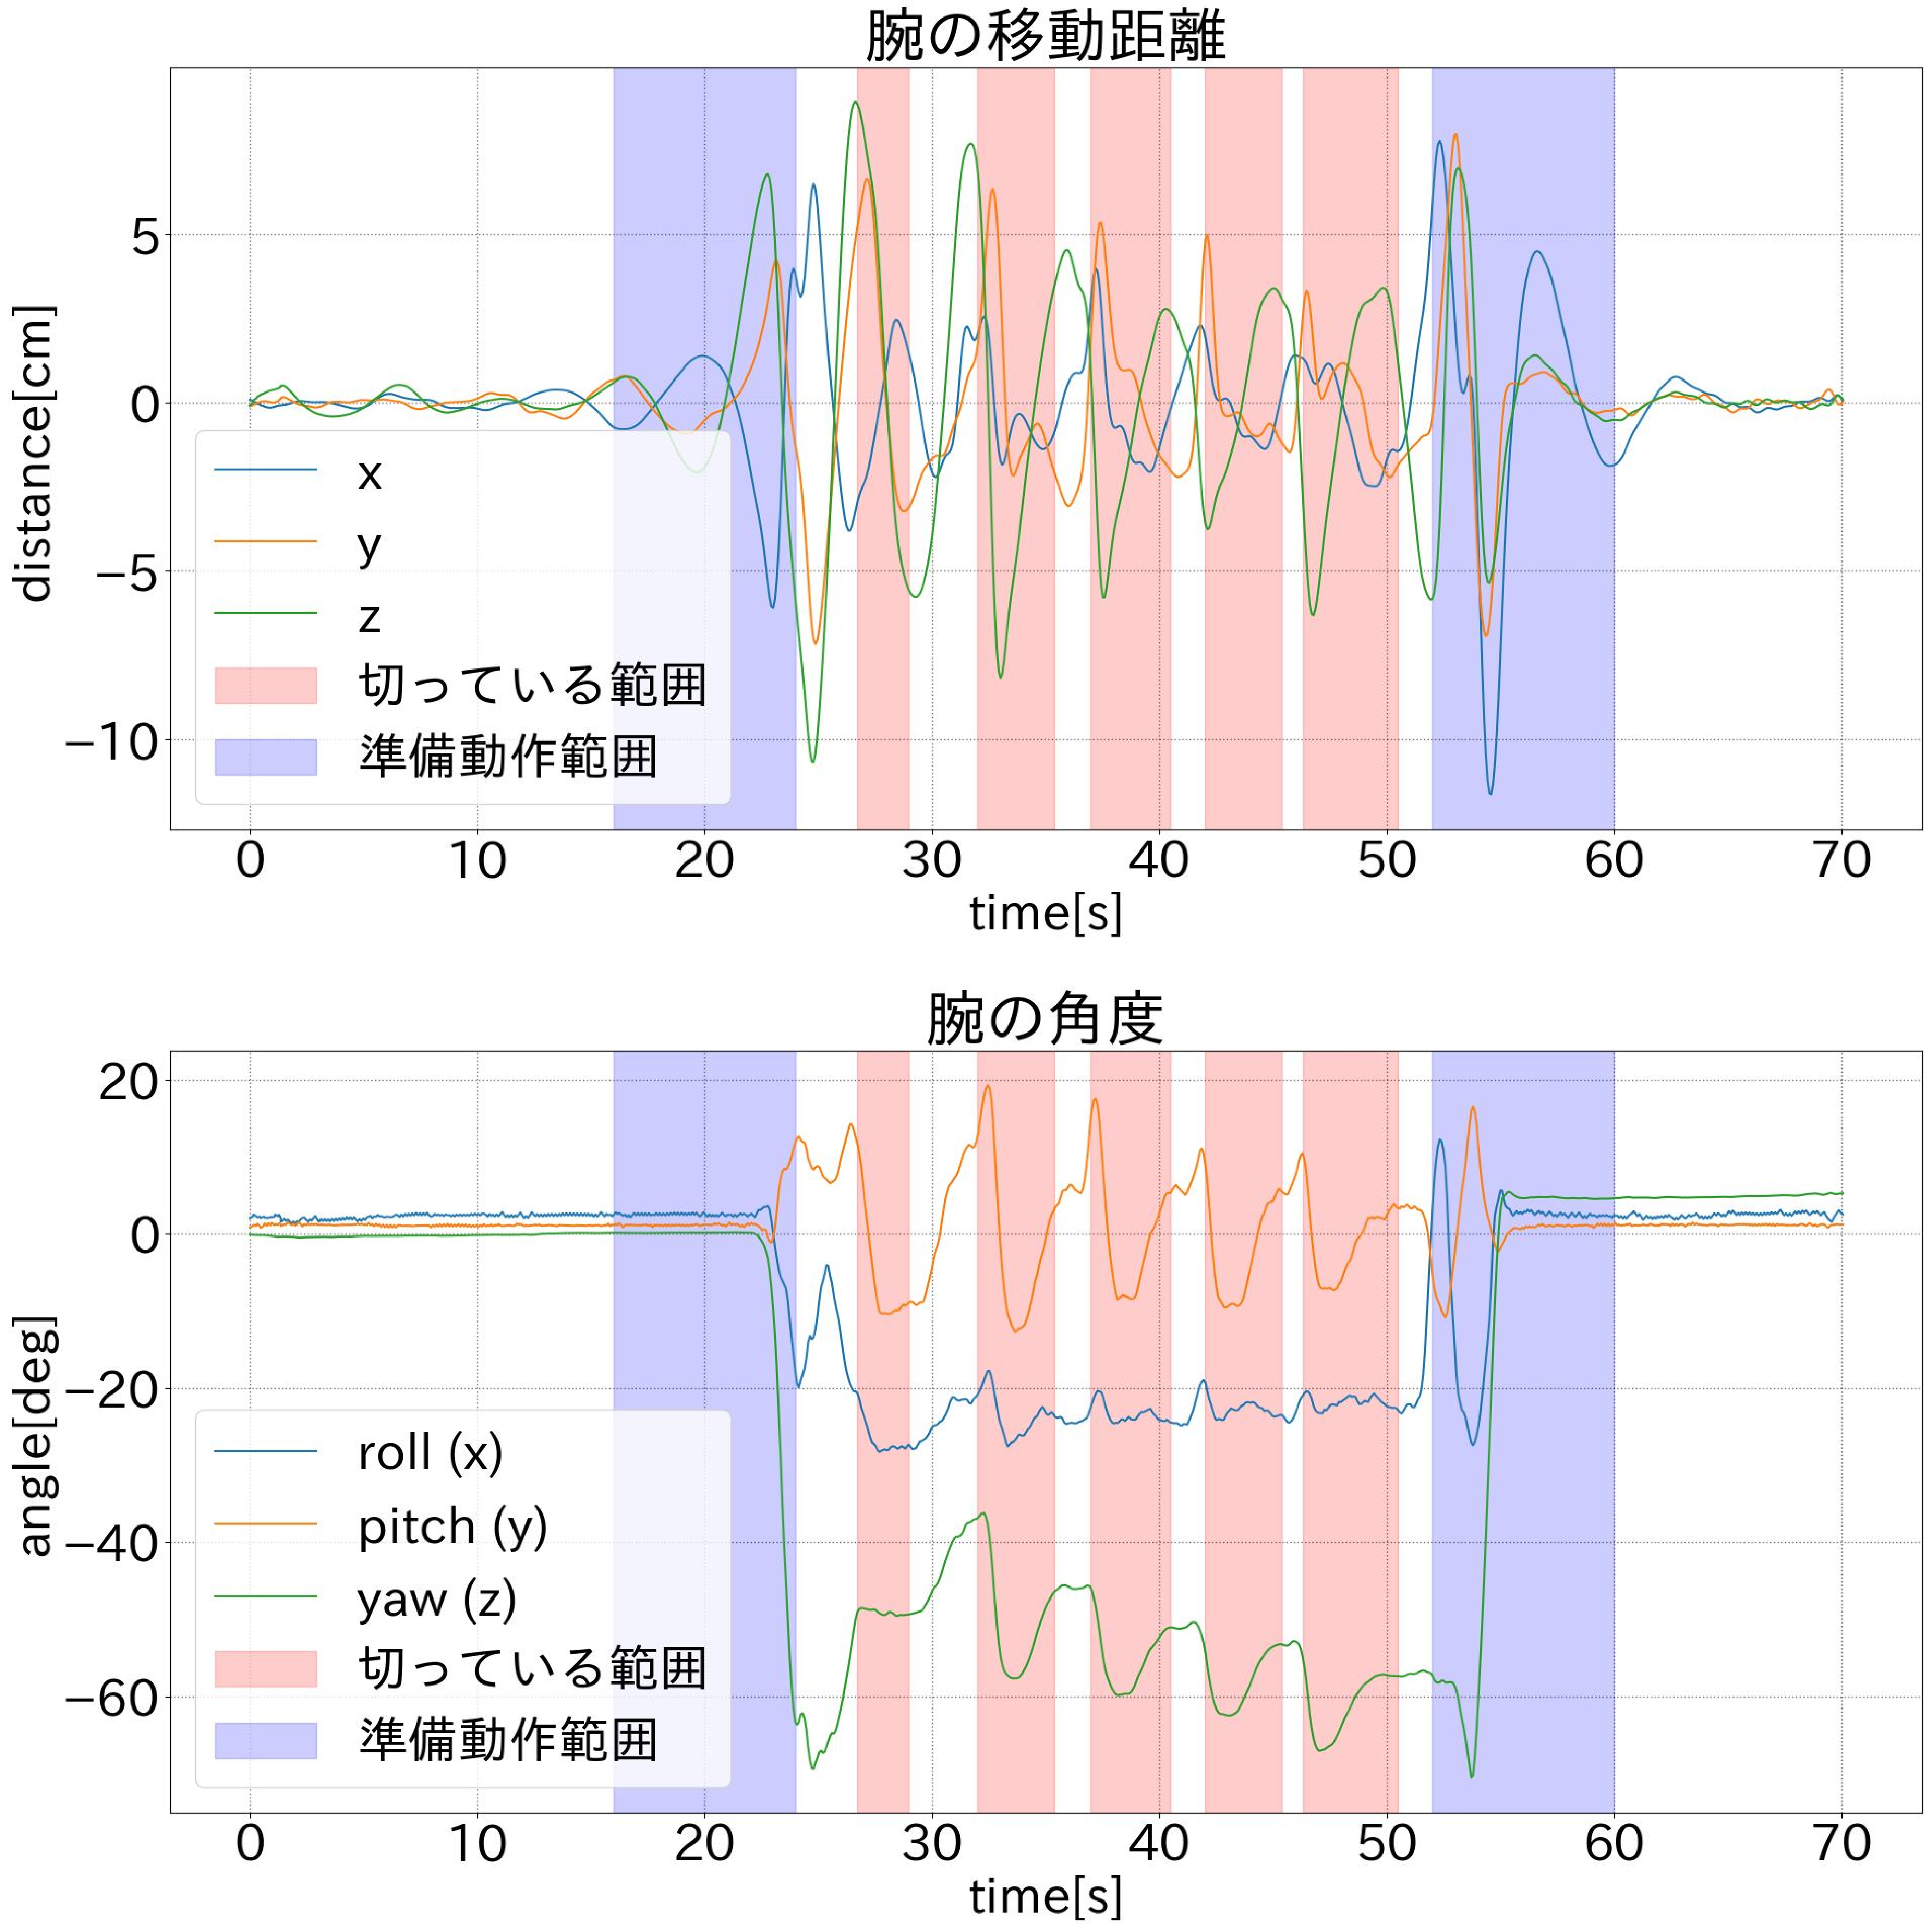
\includegraphics[width=75 mm]{images/fig3.pdf}
	\caption{積分による誤差と誤差の軽減}
	\label{fig:3}
\end{figure}

\subsection{特徴量の抽出}
推定した3次元の動きをもとに特徴量の抽出を行う.
刺身を切る動作は奥から手前に包丁を引く.
この動きはY軸方向の移動として検出される.
そこで極値処理を行い一番奥に包丁を構えた動作から包丁を引き切る動作までを一回の切り込みと定める.
また,その際かかった時間の平均値を切るペースとする.
一番奥に構えたところから包丁を引き切ったところまでの区間内での角度の平均を求める.
区間内での平均の角度から一回の切り込みにおける刃の角度を求める.

切った回数が他の人より多い場合は切っ
た食材の幅が小さい可能性があり,逆に少ない場合は幅が大きい可
能性がある.切るペースが他より早い場合は手際が良く, 逆に遅
い場合は手際が悪いと評価できる.包丁を入れた角度は, 切る手法の推定に利用できる.
刺身を切る動作の中には刃の角度をつけずに厚めに切る平造りや,斜めに刃を入れて断面を広く切るそぎ切りなどがある.
これらの切り方は主に刃を入れる角度の違いによるものであるため,刃の角度から切り方を推定できる.
このように抽出した特徴量から調理技能の評価を行う.
